\documentclass{article}
\usepackage{graphicx} % Required for inserting images

\begin{document}
 
\title{Proyecto: Intérprete Aritmético}
\author{Análisis y diseño de algoritmos} 
\date{Septiembre 2023}

\maketitle
\begin{figure}[h] 
	\centering 	
\includegraphics[width=0.5\linewidth]{Escudo UP.png}
	\label{fig:Gráfica 3}
\end{figure}

\begin{center}
\Large Integrantes del equipo:\\
\end{center}

\begin{center}
\large Natalia Malpica Blackaller \\
\large Leyre Anayantzin Ramírez Nieto \\
\large Alen Jerson Solis Ruíz
\end{center}

\begin{center}
    \Large Profesor:
\end{center}

 \begin{center}
     \large Carlos Prieto López
 \end{center}
 
\pagebreak
\section{Índice}

\begin{itemize}
    \item Introducción
    \item Descripción y análisis del problema
    \item Solución propuesta
    \item Algoritmo
    \item Diagramas de flujo
    \item Instrucciones para utilizar el programa
\end{itemize}

\pagebreak
\section{Introducción}
\normalsize Este documento pertenece al primer proyecto del semestre 1238.\\ Fue realizado en equipo, cuyos integrantes somos Natalia Malpica Blackeller, Leyre Anayantzin Ramírez Nieto y Alen Jerson Solís Ruíz; cada integrante del equipo aportó una tercera parte, es decir el 33.33\%, del trabajo para lograr lo que sería nuestra entrega final.\\ Realizamos nuestro trabajo en conjunto durante horas libres y tiempo de clase que nos fue concedido por nuestro profesor, para la realización del mismo utilizamos lo aprendido en clases y las herramientas digitales que en las mismas se nos proporcionaron.\\ A continuación, presentaremos el desglose de nuestro trabajo.

\pagebreak
\section{Descripción y análisis del problema} 
\normalsize Lo que se nos pide realizar es una especie de calculadora que solo recibe del usuario las operaciones de suma y de multiplicación, por lo que solo va a poder recibir los siguientes caracteres permitidos:
\begin{equation}\label{caracteres permitidos} 
\[Números: \ (0, 1, 2, 3, 4, 5, 6, 7, 8, 9)\]
\[Punto \ decimal \ (Ejemplo: 4.5, 2.0, 8.9, etc.)\]
\[Paréntisis \ () \]
\[Signo \ de \ suma \ (+)\]
\[Signo \ de \ multiplicación \ (*)\]
\end{equation}
\normalsize En primera instancia tiene que determinar si la operación que le proporciona el usuario es válida.\\ Entonces tenemos dos casos:\\
\normalsize \\1. La expresión es válida\\ 2. La expresión no es válida porque generó un error\\
\large\textbf{\\Caso 1: } 
\normalsize \\La expresión proporcionada cumple con lo siguiente:
\begin{enumerate}
    \item Es una cadena no vacía, significa que si contiene elementos con los que se pueda realizar alguna operación.
    \item Usa sólo caracteres válidos, siendo los siguientes: números, punto (para agregar números con decimal), signo de suma (+), signo de multiplicación (*) y paréntisis. 
    \item En caso incluir paréntesis, tiene la cantidad de pares correctos. Es decir, no sobran ni faltan paréntisis.
\end{enumerate}
\normalsize En caso de cumplir con lo anterior, se va a poder evaluar la operación para obtener su resultado.\\
\large\textbf{\\Caso 2: } 
\normalsize \\La expresión proporcionada cumple con lo siguiente:
\begin{enumerate}
    \item Es una cadena vacía, significa que no contiene elementos con los que se pueda realizar alguna operación.
    \item Incluye caracteres inválidos, siendo los siguientes: letras,  signos diferentes a los de suma (+) y/o multiplicación (*), paréntisis impares ó algún otro caracter que no sea de los permitidos. \ref{caracteres permitidos}
    \item En caso incluir paréntesis, no tiene la cantidad de pares correctos. Es decir,  sobran o  faltan paréntisis.
\end{enumerate}
\normalsize En caso de cumplir con lo anterior, no será posible evaluar la operación y  se generará un error explicando lo ocurrido.

\section{Solución propuesta}
\normalsize Nuestro intérprete aritmético está compuesto por 9 funciones que pueden dividirse en tres grupos. En primer lugar, está la función que permite la interacióncon el usuario, siendo la entrada de la expresión a evaluar. Después,  la función principal,  la cual  verifica si una cadena contiene una expresión aritmética válida y de ser así, la interpreta. Finalmente, tenemos 8 funciones que auxilian a la función principal y le permiten validar distintos casos y lanzar errores de ser necesario. A continuación se detalla   cada una de dichas funciones:
\begin{enumerate}
    \item \textbf{Función marcaError():} Señala  al usuario  dónde se encuentra un error, en caso de que la cadena proporcionada  no cumpla con las especificaciones.
    
    \item \textbf{Función eliminarCaracteresIgnorados():} Esta función se deshace  de los caracteres que no afectan la expresión, como espacios, tabuladores y saltos de línea. 
    
    \item \textbf{Función parentesisValidos():} Esta función se encarga de verificar si el uso de paréntesis en la cadena dada es adecuado. Esto implica que no se cierren paréntesis antes de abrirse y que al final de la expresión se hayan abierto exactamente la misma cantidad que cerrado.
    
    \item \textbf{Función caracteresValidos():} Comprueba que una cadena contenga únicamente caracteres permitidos, sean dígitos, punto decimal, paréntesis, o signos de suma y multiplicación.
    
    \item \textbf{Función numero():} Verifica que una cadena esté compuesta únicamente por dígitos y a lo más un punto decimal. Es decir, que represente a un número en su expresión decimal.
    
    \item \textbf{Función subexpresionBase():} Verifica que las expresiones base contengan un número, el cual puede estar precedido por '(' o seguido de ')'.
    
    \item \textbf{Función subexpresionesNoVacias():} Esta función va a ir partiendo la operación cada vez que haya un signo (+) o (*), además va a ir checando que si haya subexpresiones válidas.
    
    \item \textbf{Función interpreteAritmetico():} Esta función va a ir llamando a las funciones anteriores para checar que cumpla con lo solicitado y así, poder analizarlos como expresiones matemáticas.
    
    \item \textbf{Función entrada():} Guarda la expresión dada por usuario en una cadena que va ser analizadda por las demás funciones para verificar que sea una expresión matemática válida.
    
\end{enumerate}

\pagebreak
\section{Algoritmo}
\normalsize En esta sección se presenta el desglose de lo que sería el algoritmo que sigue cada una de nuestras funciones.
\subsection{Función marcaError()}
\normalsize Dada una cadena y la posición del error, concatena una nueva cadena donde se señala.
\begin{enumerate}
    \item Inicio.
    \item Recibe una cadena y la posición del caracter que contiene un error guardada en la variable caracterEnLinea.
    \item Crea una cadena vacía llamada nuevaCadena.
    \item Agrega todos la caracteres previos al error a la cadena nueva.
    \item Concatena $<$, el caracter erróneo y $>$ a la nueva cadena.
    \item Concatena uno a uno a la nueva cadena todos los caracteres posteriores al erróneo en la cadena original.
    \item Regresa la cadena nueva.
    \item Termina la función.
\end{enumerate}

\subsection{Función eliminarCaracteresIgnorados()}
\normalsize En esta función eliminamos los caractéres que no afectan la validez de la cadena ni afectan el valor de la expresión.
\begin{enumerate}
    \item Inicio.
    \item Recibe una cadena.
    \item Crea una lista de los caracteres ignorados: espacio (""), tabulador ("\backslash t") y salto de línea ("\backslash n"),
    \item Crea una nueva cadena vacía.
    \item Para cada caracter a  en la cadena:
    \begin{enumerate}
        \item Crea un booleano noIgnorado  = 1  (más adelante, 0 representará que va a ser ignorado y eliminado, mientras que 1 significa que permanecerá en la cadena).
        \item Para todo caracter b  en la lista de caracteres ignorados:
        \begin{enumerate}
            \item Si a == b, entonces noIgnorados = 0 (el caracter a es un de los caracteres que vamos a eliminar).
        \end{enumerate}
        \item Si noIgnorado == 1, entonces, concatena el caracter a al final de la nueva cadena (de lo contrario no se agrega a la cadena nueva).
    \end{enumerate}
    \item Regresa a la nueva cadena (igual a la original sin los caracteres ignorados).
    \item Fin.
\end{enumerate}

\subsection{Función parentesisValidos()}
\normalsize Esta función se encarga de verificar si el uso de paréntesis en la cadena dada es adecuado. Esto implica que no se cierren paréntesis antes de abrirse y que al final de la expresión se hayan abierto exactamente la misma cantidad que cerrado.
\begin{enumerate}
    \item Inicio.
    \item Recibe una cadena de texto.
    \item Crea una variable c=0 que nos permitirá llevar la cuenta de los paréntesis abiertos y cerrados.
    \item Crea una variable caracterEnLinea = 1, que guardará la posición actual en la cadena (con ello podremos indicar dónde hay errores de ser así).
    \item Para cada caracter a  en la cadena:
    \begin{enumerate}
        \item Si a  == ‘(‘, entonces suma 1 a c.
        \item Si a  == ‘)‘, entonces resta 1 a c.
        \item Si c $<$ 0, esto significa que se han cerrado más paréntesis de los que se han abierto, así que devuelve un error y termina la función.
        \item Suma 1 a caracterEnLinea.
    \end{enumerate}
    \item Si c es distinto de cero después de haber recorrido toda la cadena, significa que no todos los paréntesis que se abrieron fueron cerrados, por lo tanto lanza un error y termina la función.
    \item Termina la función.
\end{enumerate}

\subsection{Función caracteresValidos()}
\normalsize En esta función verificamos que la cadena no contenca ningún caracter que el intérprete aritmético no acepte.
\begin{enumerate}
    \item Inicio.
    \item Recibe una cadena.
    \item Crea una lista con los caracteres válidos: '0', '1', '2', '3', '4', '5', '6', '7', '8', '9', '.', '(', ')', '*', '+'
    \item Crea una variable caracterEnLinea = 1, que guardará la posición actual en la cadena (con ello podremos indicar dónde hay errores de ser así).
    \item Para cada caracter a  en la cadena:
    \begin{enumerate}
        \item Para cada caracter b  en la lista de caracteres válidos: 
        \begin{enumerate}
            \item Si  a == b,  pasa a la siguiente iteración de a.
        \end{enumerate}
        \item Si se recorrió toda la lista de caracteres válidos y a no coincidió con ninguno, entonces lanza un error y termina la función.
        \item Suma 1 a caracterEnLinea.
    \end{enumerate}
    \item Termina la función.
\end{enumerate}

\subsection{Función numero()}
\normalsize Verifica si una cadena es únicamente un número. Para ello debe estar conformada por dígitos y a lo más un punto decimal.
\begin{enumerate}
    \item Inicio.
    \item Recibe:
    \begin{enumerate}
        \item cadena: una cadena de texto.
        \item num:  un fragmento de la cadena que queremos verificar que sea un número.
        \item inicionumero: La posición del primer caracter de num  con respecto a la cadena.
    \end{enumerate}
    \item Crea puntos = 0, un contador de la cantidad de puntos en num (no puede tener más de un punto decimal).
    \item Crea una variable tam que guarde el tamaño de num.
    \item Crea una lista digitos que contiene los caracteres válidos para un número (dígitos y punto decimal): '0', '1', '2', '3', '4', '5', '6', '7', '8', '9', '.'
    \item Sea i = 1 un iterador para recorrer los caracteres de  num.
    \item Mientras i $<$= tam:
    \begin{enumerate}
        \item Si num[i] == ‘.’ :
        \begin{enumerate}
            \item Suma 1 a puntos.
            \item Si puntos $>$ 1, lanza un error y termina la función (pues un número no puede contener más de un punto decimal).
        \end{enumerate}
        \item De lo contrario:
        \begin{enumerate}
            \item Sea j = 1 un iterador para recorrer dígitos.
            \item Mientras j $<$= length(digitos):
            \begin{enumerate}
                \item Si digitos[j] == num[i], entonces asigna j = length(digitos) + 1 (con ello j es mayor que length(digitos) y se detiene el ciclo).
                \item Si j == length(digitos) y num[i] != digitos[j], esto significa que se llegó al final del ciclo y num[i] no coincide con ninguno de los caracteres válidos. Por lo tanto, lanza un error y termina la función.
                \item Suma 1 a j para pasar a la siguiente iteración.
            \end{enumerate}
            \item Suma 1 a i para pasar a la siguiente iteración.
        \end{enumerate}
        \item Si, tam == 1 y puntos == 1, esto significa que num == “.” lo cual no es un número válido. Por lo tanto, lanza un error y termina la función.
    \end{enumerate}
    \item Termina la función.
\end{enumerate}

\subsection{Función subexpresionBase()}
\normalsize Las expresiones base deben contener exactamente un número. Antes del número pueden haber paréntesis abiertos y después, paréntesis cerrados.
\begin{enumerate}
    \item Inicio.
    \item Recibe:
    \begin{enumerate}
        \item cadena: una cadena de texto.
        \item subexpresion1: un fragmento de la cadena que queremos verificar que sea una subexpresión base.
        \item inicioSubexpresión: La posición del primer caracter de subexpresion1  con respecto a la cadena.
    \end{enumerate}
    \item Crea la variable inicioNumero = 0 (guardará la posición en que los caracteres de la subexpresión dejen de ser ‘(‘ y deba comenzar el número).
    \item Si length(subexpresion1) == 0, esto significa que que está vacía (y por ello no es una subexpresión base). Por ello, lanzar un error y terminar la función.
    \item Sea i = 1 un iterador para recorrer la subexpresión.
    \item Mientras i $<$= length(subexpresion1):
    \begin{enumerate}
        \item Si subexpresion1[i] == '(':
        \begin{enumerate}
            \item Si i == length(subexpresion1), esto significa que desde el inicio de la subexpresión, hasta el final todos los caracteres son ‘(‘. Por lo tanto, la subexpresión no contiene ningún número y no es una subexpresión base, así que lanza un error y termina la función.
            \item Si subexpresion1[i] == ')', entonces se cierra un paréntesis antes del número, lo cual no está permitido, así que lanza un error y termina la función.
            \item De lo contrario, si  subexpresion1[i] no es un paréntesis, debe ser parte del número. Por lo tanto, inicioNumero = i y termina el ciclo.
        \end{enumerate}
        \item Suma 1 a i para pasar a la siguiente iteración.
    \end{enumerate}
    \item Crea una variable finNumero = inicioNumero  (el numero debe contener al menos un dígito, por lo que finNumero es mayor o igual que inicioNumero).
    \item Mientras finNumero $<$ length(subexpresion1) el número puede contener otro caracter:
    \begin{enumerate}
        \item Si subexpresion1[finNumero + 1] != ')', entonces finNumero = finNumero + 1 (después del número no puede seguir nada distinto a paréntesis que cierran).
        \item De lo contrario, termina el ciclo (si el siguiente caracter es ‘)’, entonces ya no pertenece al número).
    \end{enumerate}
    \item Si finNumero $<$ length(subexpresion1), entonces hay caracteres en la subexpresión posteriores al número y todos deben ser ‘)’ para que sea una expresión válida:
    \begin{enumerate}
        \item Sea i = finNumero  + 1 un iterador para recorrer los caracteres restantes de la subexpresión.
        \item Mientras i $<$=  length(subexpresion1):
        \begin{enumerate}
            \item Si if subexpresion1[i] != ')', lanza un error y termina la función, pues ‘)’ es el único caracter válido después de un número.
            \item Suma 1 a i para pasar a la siguiente iteración.
        \end{enumerate}
    \end{enumerate}
    \item Asigna candidatoNumero = subexpresion1[inicioNumero:finNumero].
    \item Si numero(candidatoNumero, (inicioNumero + inicioSubexpresion  - 1), cadena) no regresa un error, entonces candidatoNumero y subexpresion1  es una subexpresión base válida.
    \item Termina la función.
\end{enumerate}

\subsection{Función subexpresionesNoVacias()}
\normalsize Esta función “fragmenta” la cadena con los caracteres ‘+’ y ‘*’. Además, verifica que que entre cada par de los caracteres anteriores, haya una subexpresión base válida (de lo contrario dicom que hay una vacía entre ellos).
\begin{enumerate}
    \item Inicio.
    \item Recibe una cadena.
    \item Crea:
    \begin{enumerate}
        \item tam  = length(cadena).
        \item posicion = 1 (nos permitirá saber en qué caracter de la cadena nos encontramos.
        \item subexpresion1 = “” (una cadena vacía).
        \item inicioNuevaSubexpresion = 1 (nos iniciará dónde comienza subexpresión que fragmentaremos de la cadena).
    \end{enumerate}
    \item Mientras posicion $<$= tam:
    \begin{enumerate}
        \item Si cadena[posicion] == '+':
        \begin{enumerate}
            \item Si posicion == 1 o posicion == tam, regresa un error y termina la función, pues una expresión válida no puede comenzar ni terminar con el caracter ‘+’.
            \item De lo contrario subexpresion1 = cadena[inicioNuevaSubexpresion: posicion - 1]  (del inicio de la nueva subexpresión que tenía guardado al caracter previo al ‘+’ que “partió” la expresión”.
            \item Corre la función subexpresionBase(subexpresion1, inicioNuevaSubexpresion, cadena) para verificar que subexpresion1 sea una subexpresión base válida.
            \item La siguiente subexpresion a la acabada de verificar comienza un caracter después del ‘+’ que "fragmentó" la expresión, entonces inicioNuevaSubexpresion = posicion + 1.
        \end{enumerate}
        \item Si cadena[posicion] == '*':
        \begin{enumerate}
            \item Si posicion == 1 o posicion == tam, regresa un error y termina la función, pues una expresión válida no puede comenzar ni terminar con el caracter ‘*’.
            \item De lo contrario subexpresion1 = cadena[inicioNuevaSubexpresion: posicion - 1]  (del inicio de la nueva subexpresión que tenía guardado al caracter previo al ‘*’ que “partió” la expresión.
            \item Corre la función subexpresionBase(subexpresion1, inicioNuevaSubexpresion, cadena) para verificar que subexpresion1 sea una subexpresión base válida.
            \item La siguiente subexpresion a la acabada de verificar comienza un caracter después del ‘*’ que “fragmentó" la expresión, entonces inicioNuevaSubexpresion = posicion + 1.
        \end{enumerate}
        \item Suma 1 a posicion para pasar a la siguiente iteración.
    \end{enumerate}
    \item Termina la función.
\end{enumerate}

\subsection{Función interpreteAritmetico()}
\normalsize Interpreta a los valores de la cadena como expresiones matemáticas si cumplen los requisitos de la función.
\begin{enumerate}
    \item Inicio.
    \item Recibe una cadena.
    \item Limpia la cadena con la función eliminarCaracteresIgnorados(cadena) y almacena el resultado en cadena.
    \item Verifica que los paréntesis de la cadena con parentesisValidos(cadena).
    \item caracteresValidos(cadena) verifica que todos que  la cadena contenga únicamente los caracteres aceptados.
    \item subexpresionesNoVacías(cadena) “parte” la cadena y verifica que cada fragmento contenga una subexpresión base válida.
    \item Si ninguna de la funciones anteriores lanzó un error, entonces la cadena contiene una expresión matemática válida:
    \begin{enumerate}
        \item La  transforma en un float  y almacenarlo en  resultado con las siguientes funciones: float(eval(Meta.parse(cadena)))
        \item Regresa resultado.
    \end{enumerate}
    \item Terminar la función.
\end{enumerate}

\subsection{Función entrada()}
\begin{enumerate}
    \item Inicio
    \item Crea cadena  = “” (una cadena vacía).
    \item Lee una línea de texto dada por el usuario y la almacena en linea.
    \item Mientras que length(linea) $>$ 0    (mientras que el usuario no ingrese una línea vacía):
    \begin{enumerate}
        \item cadena  = cadena * linea  (concatena la nueva linea con la cadena)
        \item vuelve a leer una línea del usuario y la guarda en cadena.
    \end{enumerate}
    \item Regresa cadena.
    \item Termina la función.
\end{enumerate}

\subsection{Archivo "interprete\_aritmetico"}
\begin{enumerate}
    \item Inicio.
    \item Indica al usuario las instrucciones y le piede una expresión válida.
    \item Lee la expresión del usuario mediante entrada() y la almacena en cadena.
    \item Verifica que sea una expresión válida a través de intérpreteAritmético(cadena):
    \begin{enumerate}
        \item Si la expresión es válida la almacena en resultado y la imprime.
        \item De lo contrario, regresa un error.
    \end{enumerate}
    \item Fin.
\end{enumerate}

\pagebreak
\section{Diagramas de flujo}
\normalsize A continuación presentamos los respectivos diagramas de flujo de las funciones que realizamos. Para una mejor comprensión realizamos un diagrama por cada función y en el que corresponde a  la \textit{Función interpreteAritmetico()} se llama a cada una de las funciones. La \textit{Función entrada()} es la que va a recibir la operación para poder ejecutar el intérprete aritmético.

\subsection{Función marcaError()}
\begin{figure}[h] 
	\centering 	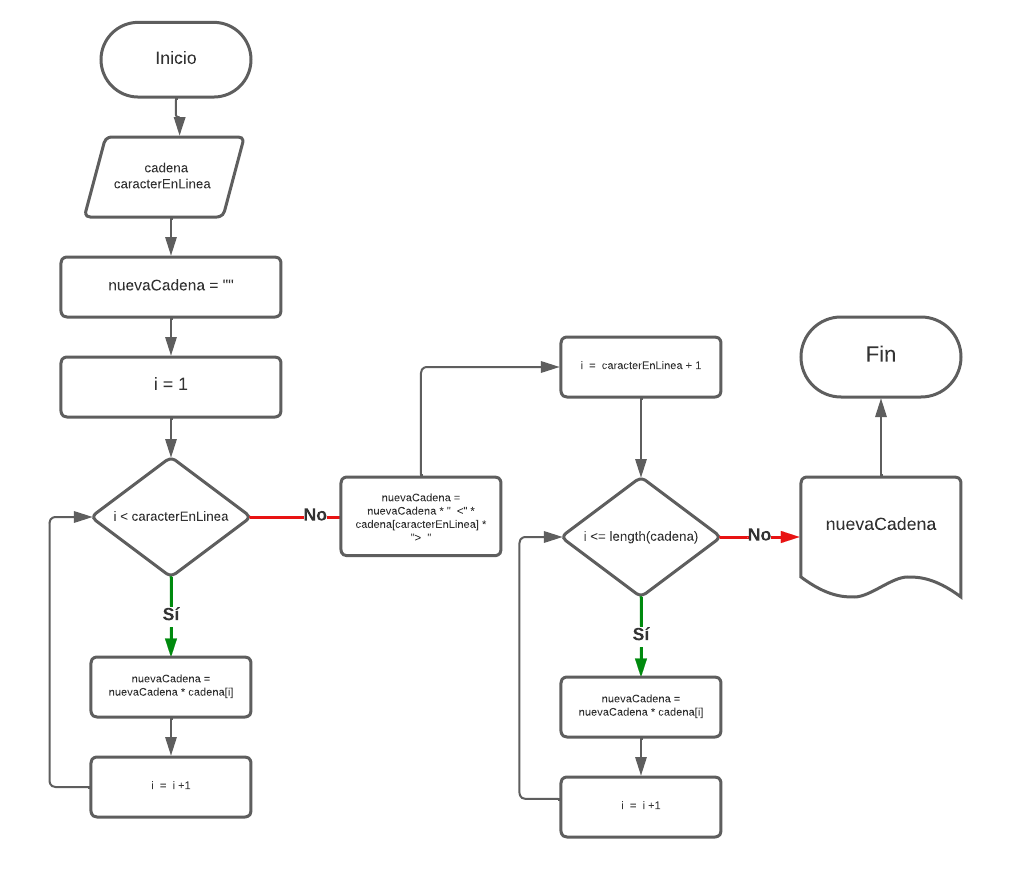
\includegraphics[width=1.25\linewidth]{Función marcaError.png}
	\label{fig:Gráfica 3}
\end{figure}

\pagebreak
\subsection{Función eliminarCaracteresIgnorados()}
\begin{figure}[h] 
	\centering 	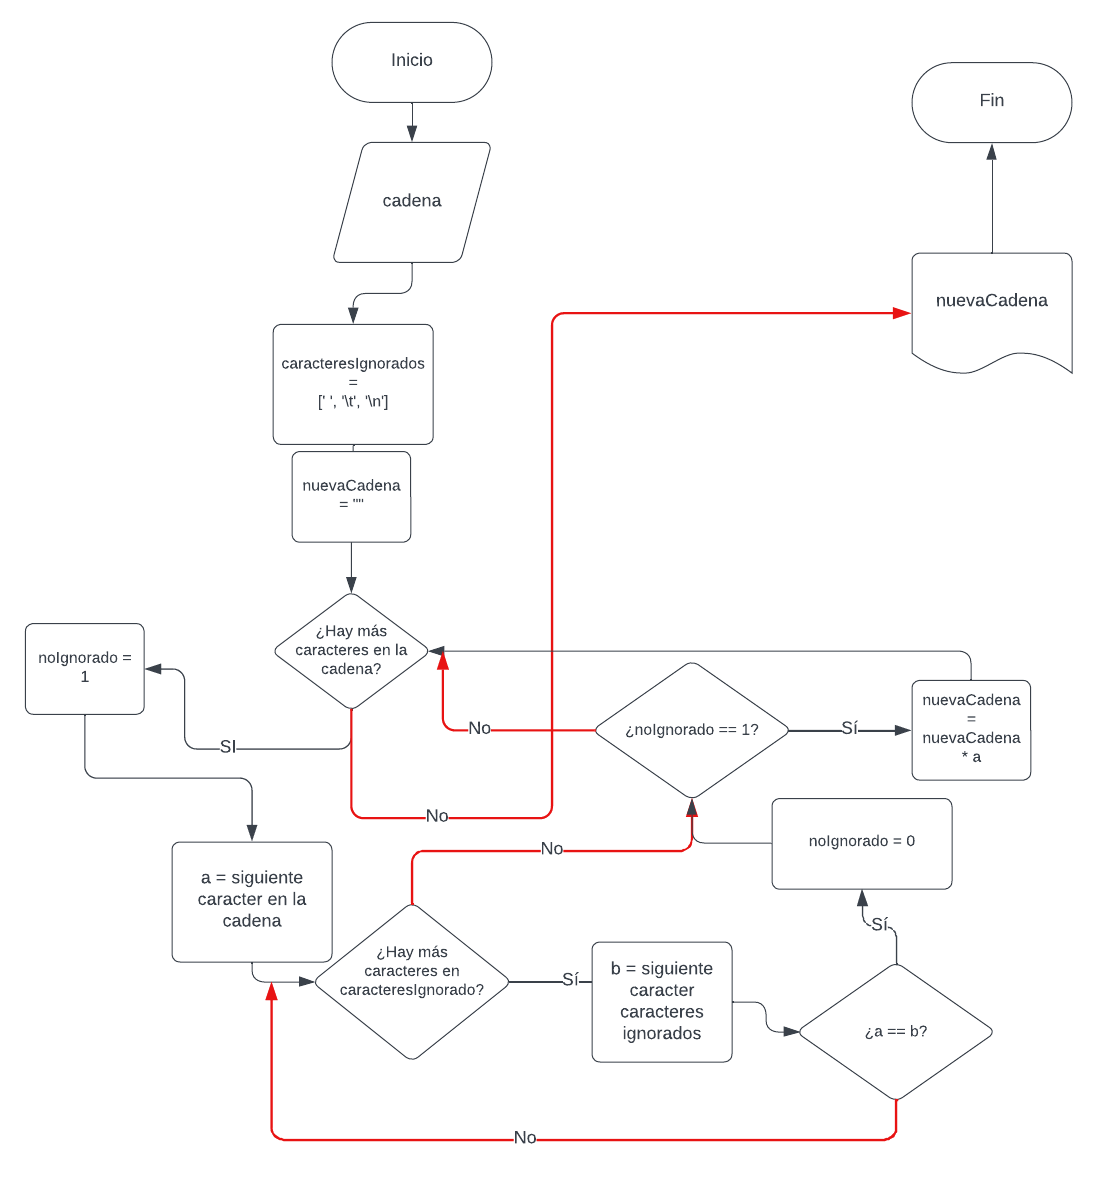
\includegraphics[width=1\linewidth]{Función eliminarCaracteresIgnorados.png}
	\label{fig:Gráfica 3}
\end{figure}

\pagebreak
\subsection{Función parentesisValidos()}
\begin{figure}[h] 
	\centering 	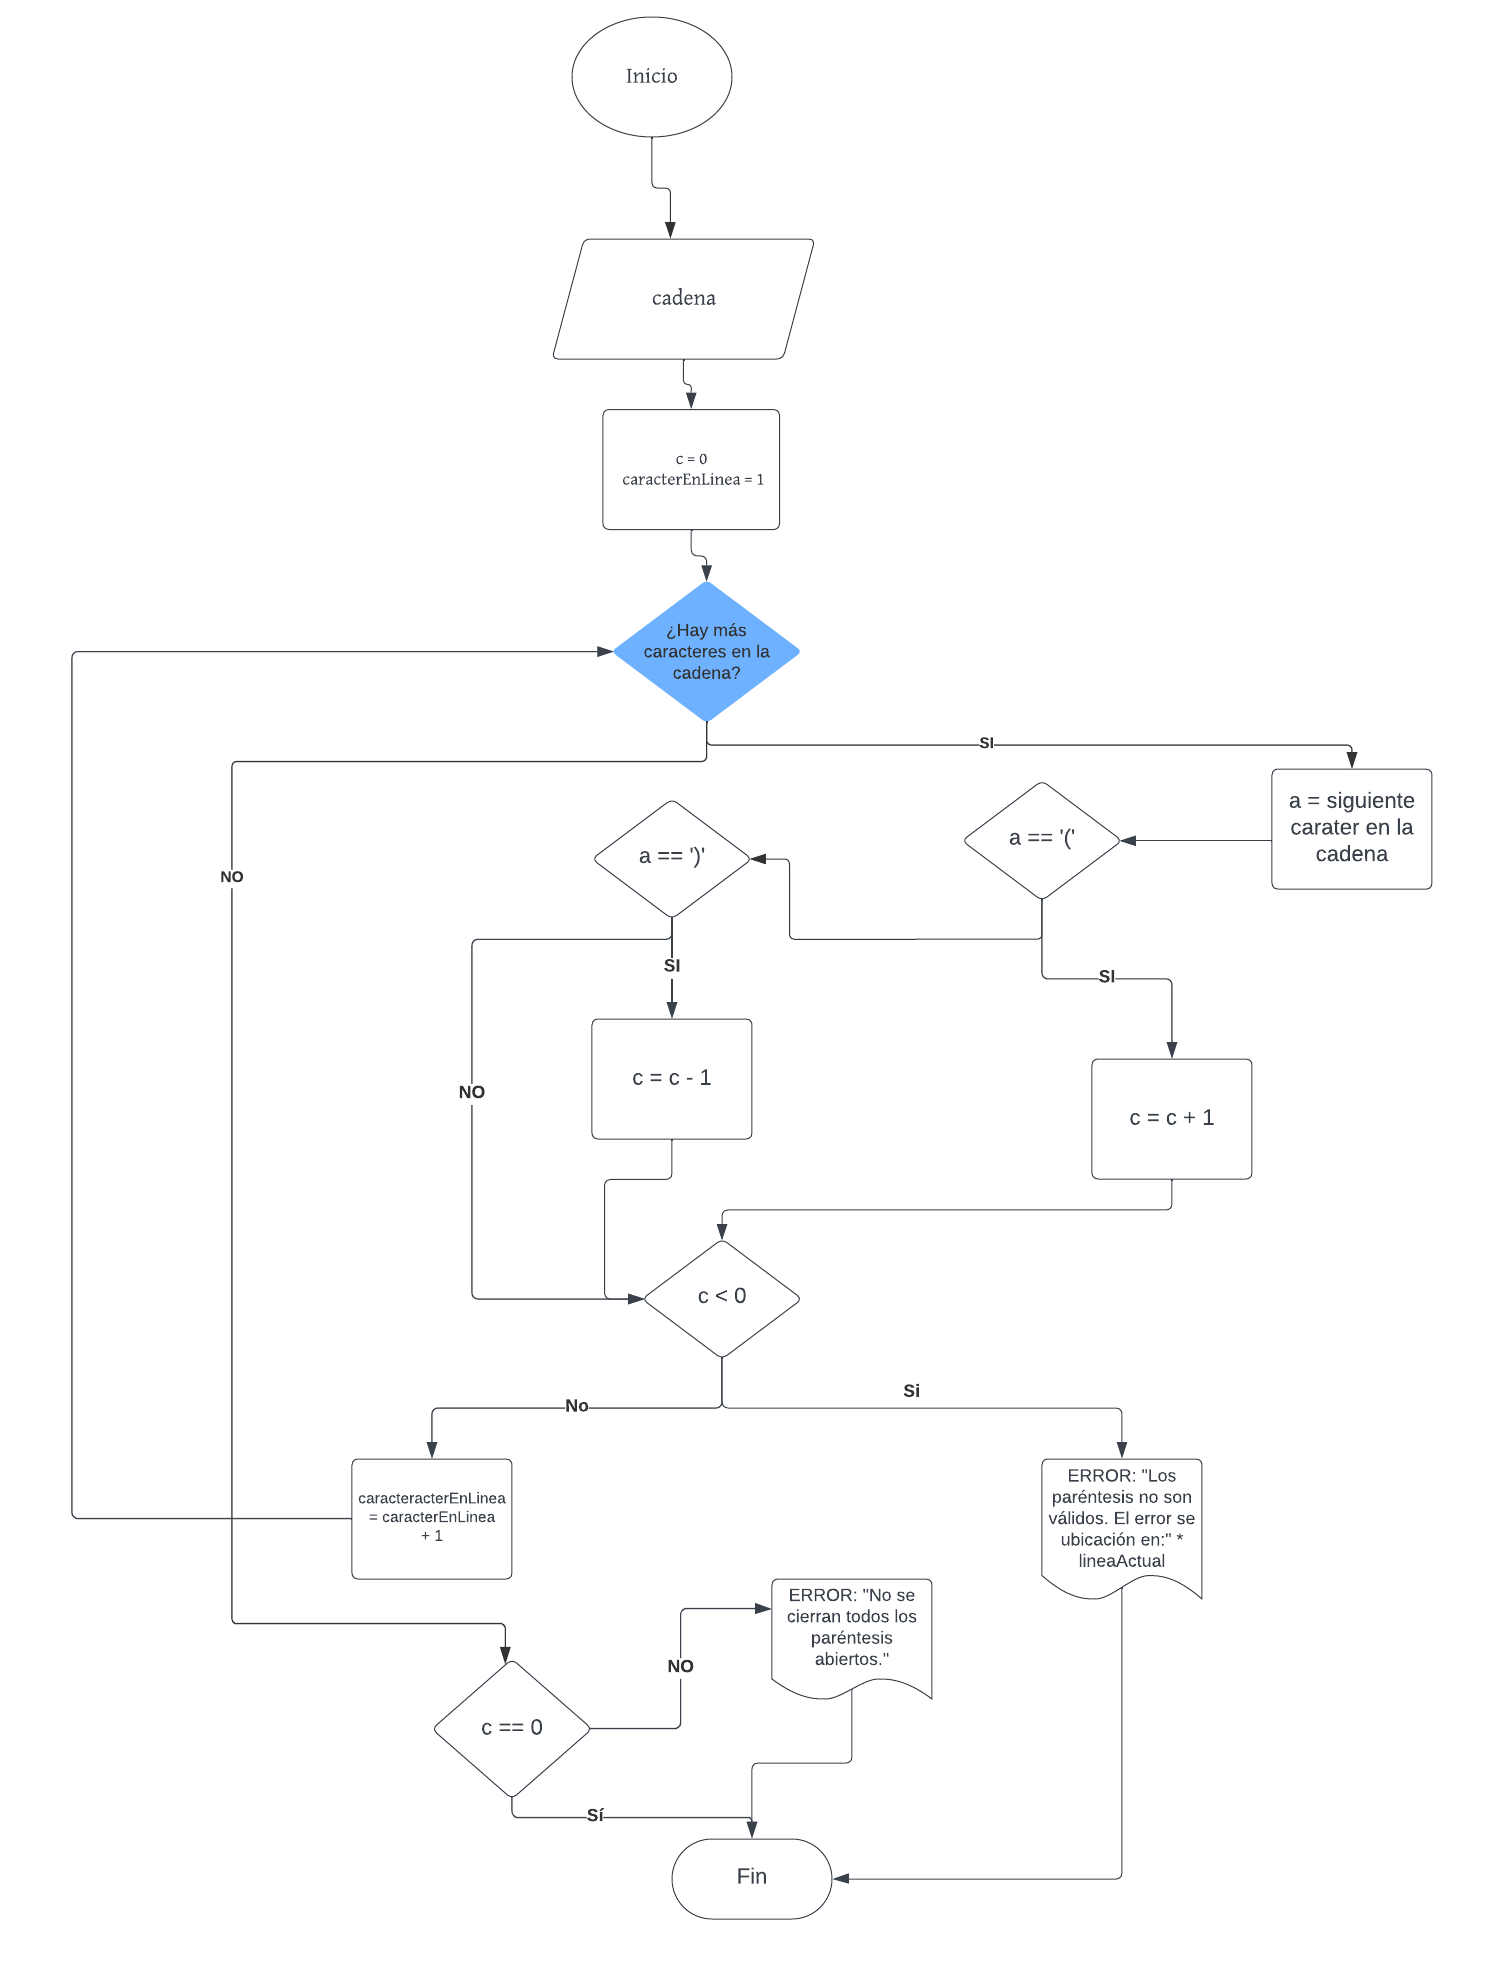
\includegraphics[width=0.94\linewidth]{Función parentesisValidos.png}
	\label{fig:Gráfica 3}
\end{figure}

\pagebreak
\subsection{Función caracteresValidos()}
\begin{figure}[h] 
	\centering 	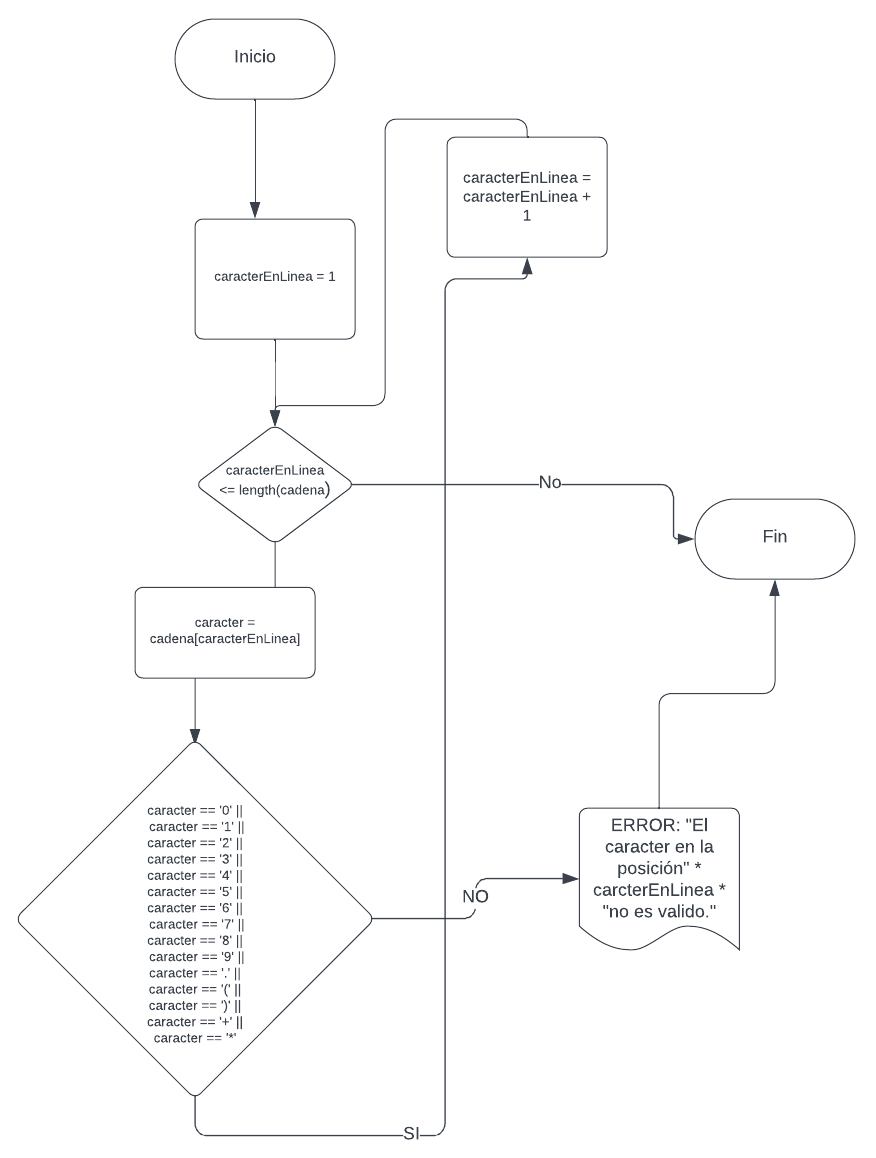
\includegraphics[width=0.9\linewidth]{Función caracteresValidos.png}
	\label{fig:Gráfica 3}
\end{figure}

\pagebreak
\subsection{Función numero()}
\begin{figure}[h] 
	\centering 	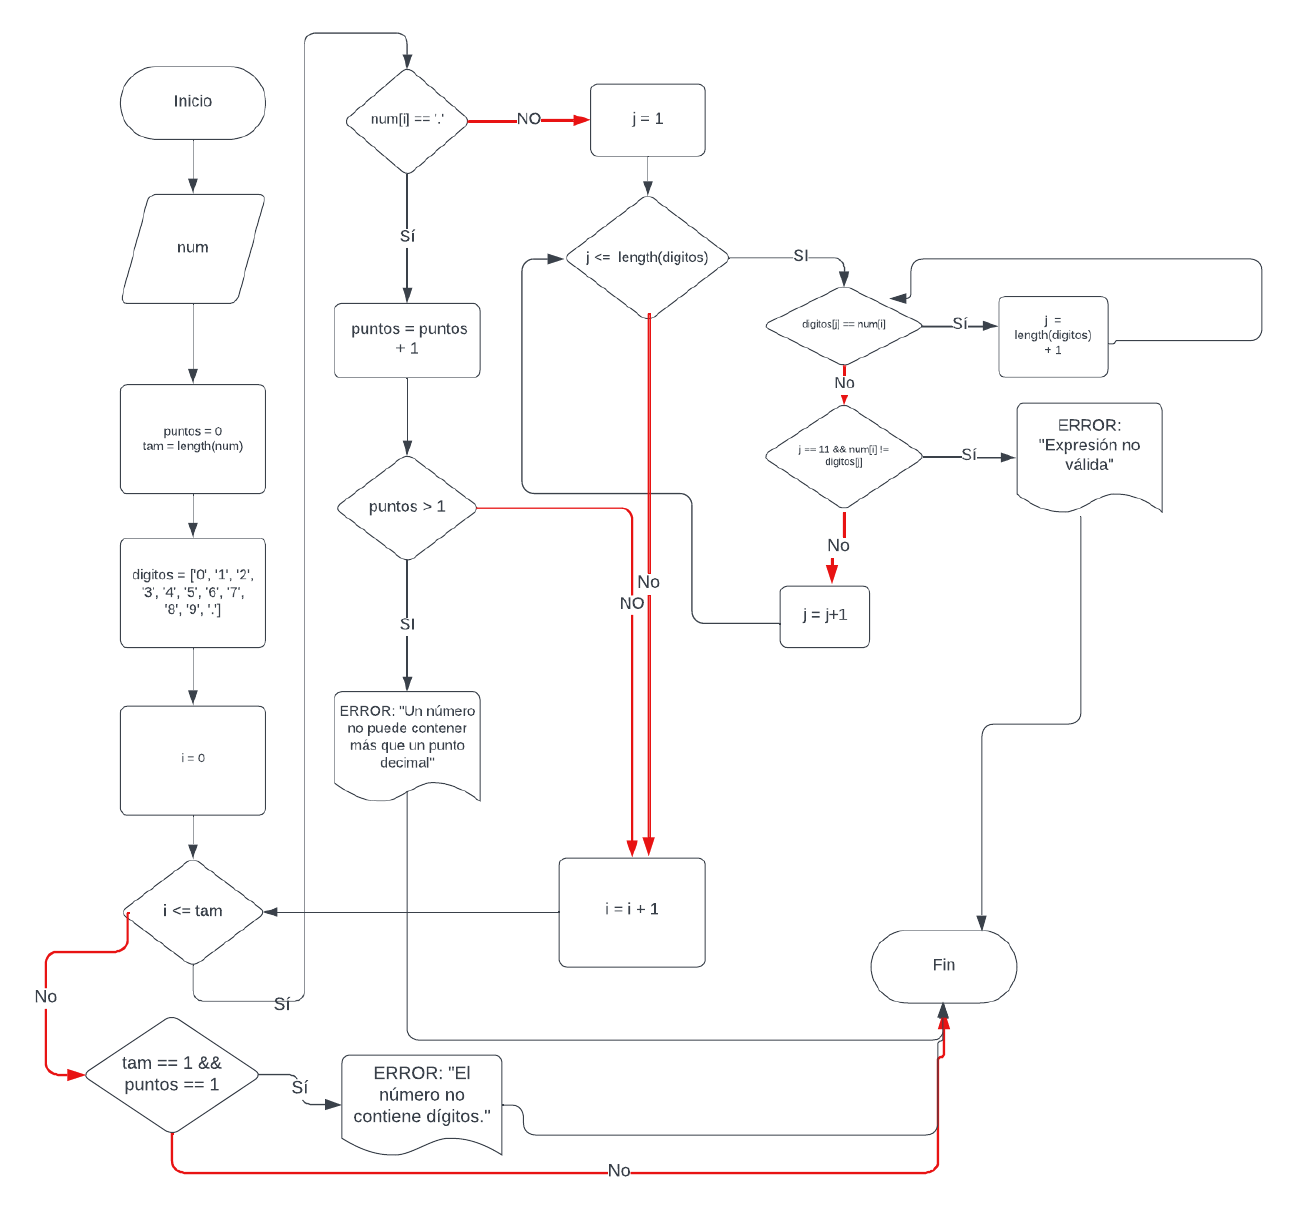
\includegraphics[width=1.25\linewidth]{Función numero.png}
	\label{fig:Gráfica 3}
\end{figure}

\pagebreak
\subsection{Función subexpresionBase()}
\begin{figure}[h] 
	\centering 	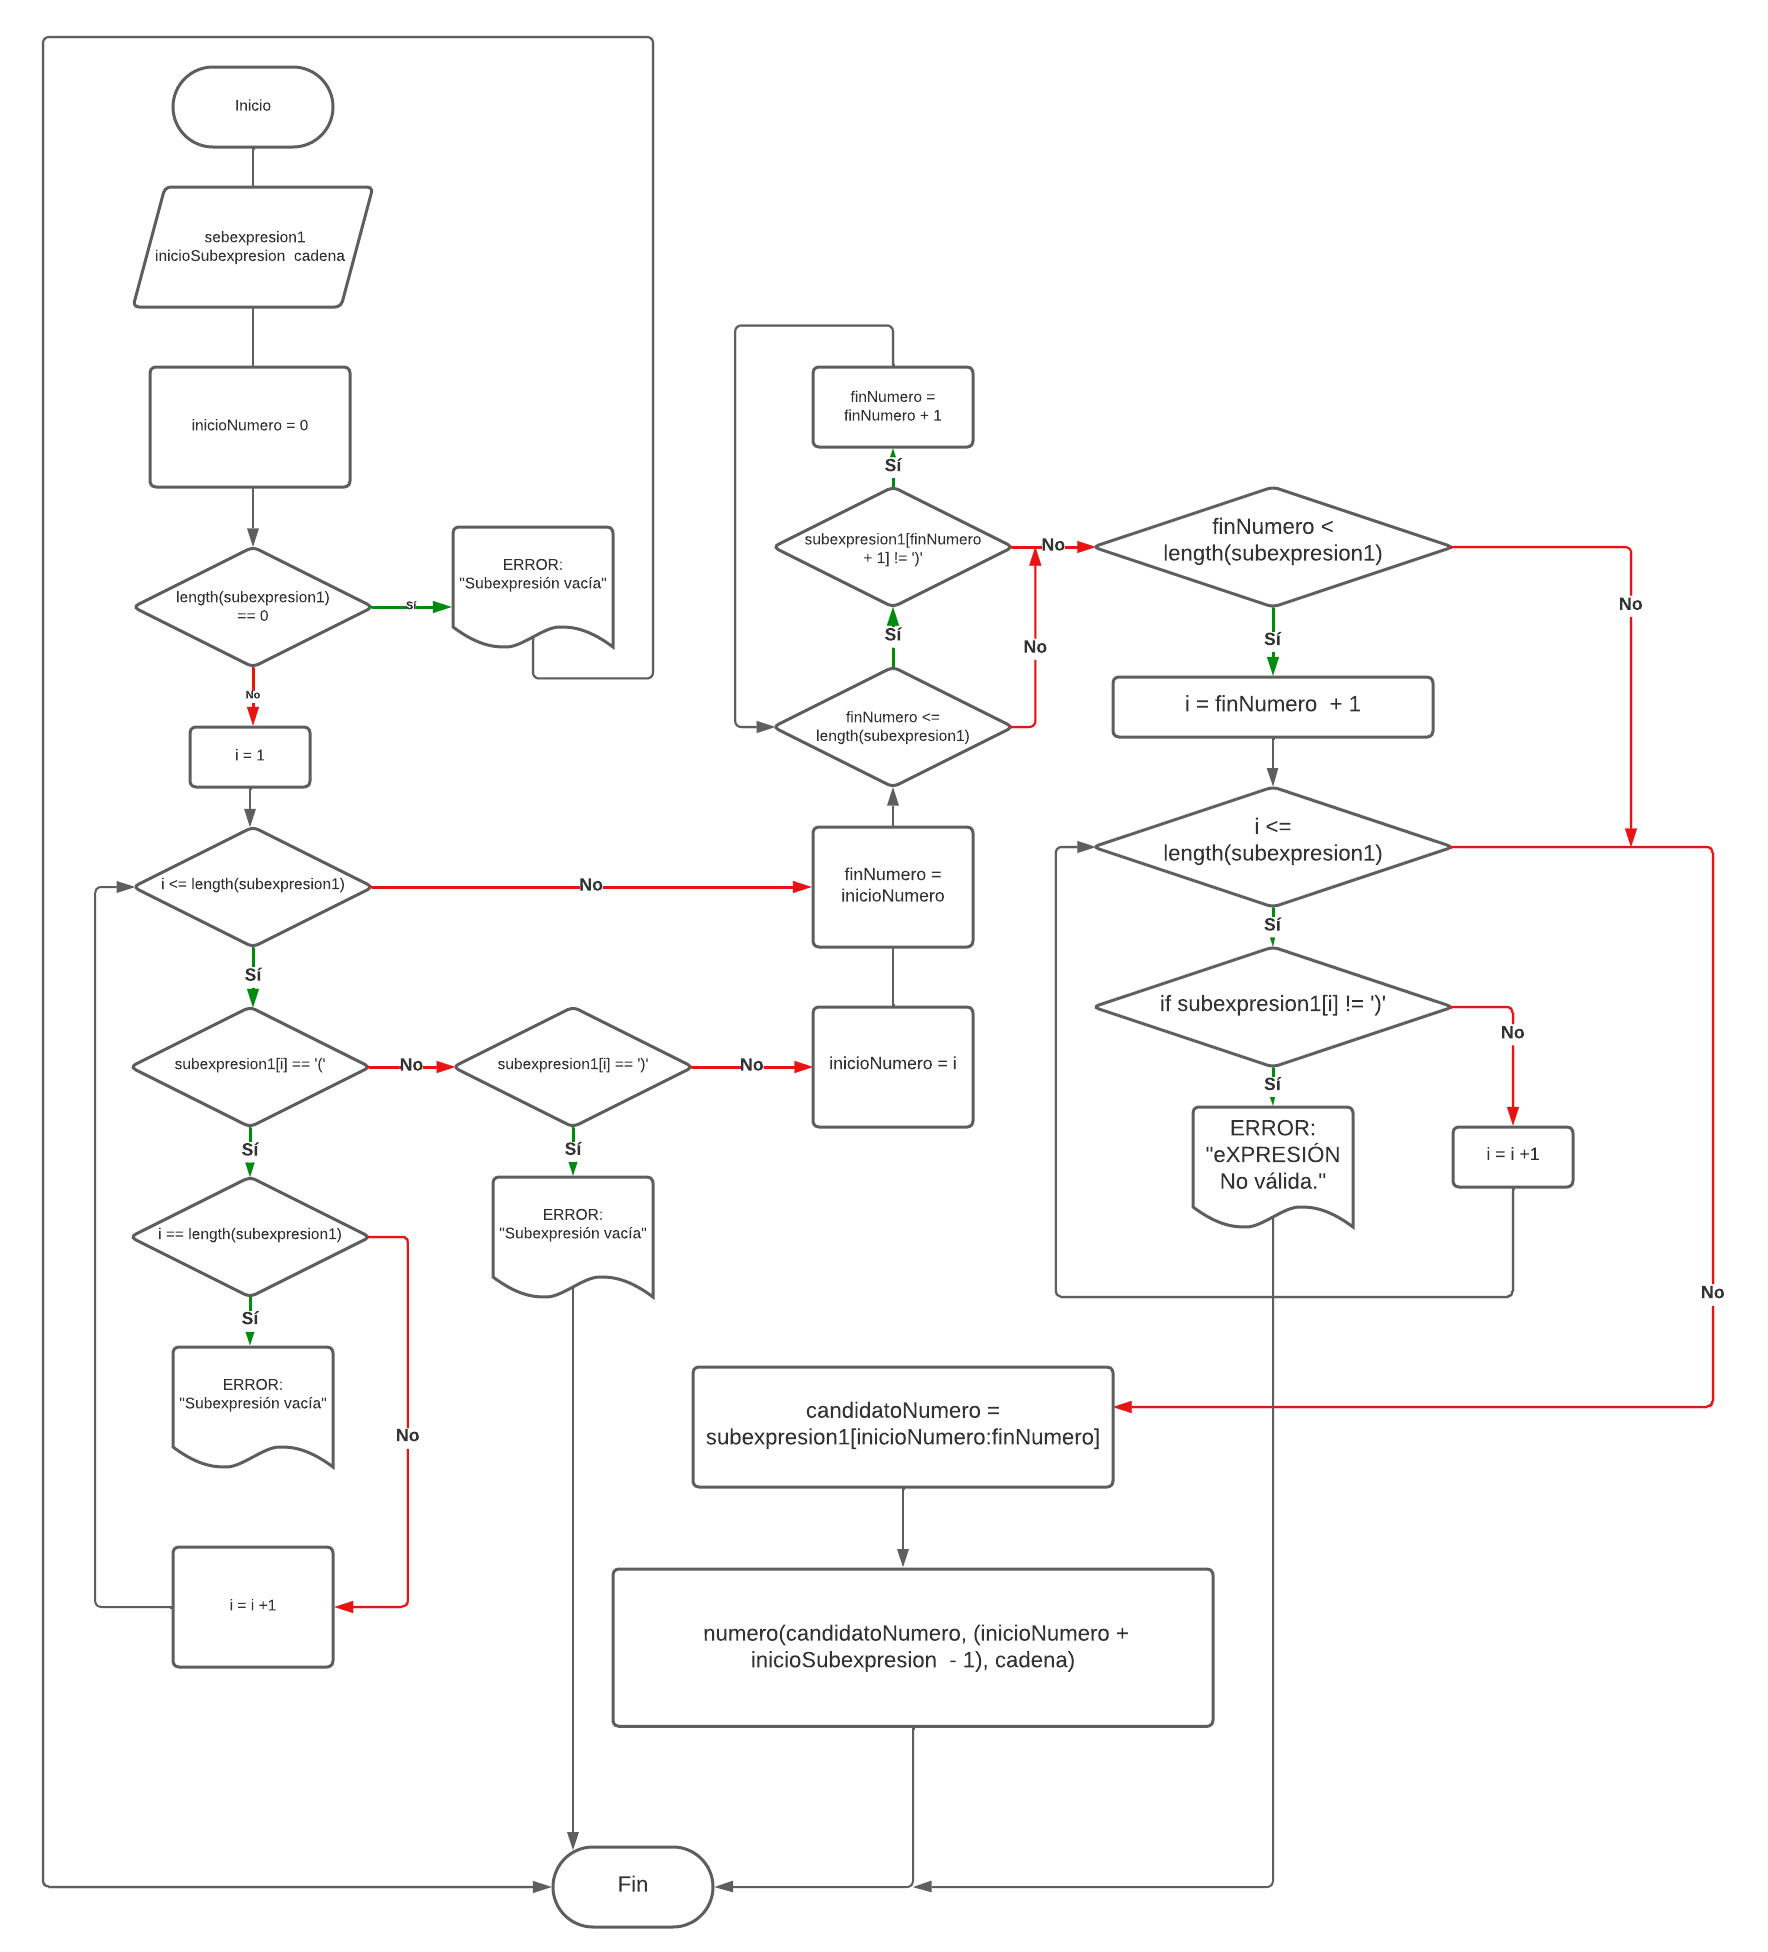
\includegraphics[width=1.09\linewidth]{Función subexpresionBase.png}
	\label{fig:Gráfica 3}
\end{figure}

\pagebreak
\subsection{Función subexpresionesNoVacias()}
\begin{figure}[h] 
	\centering 	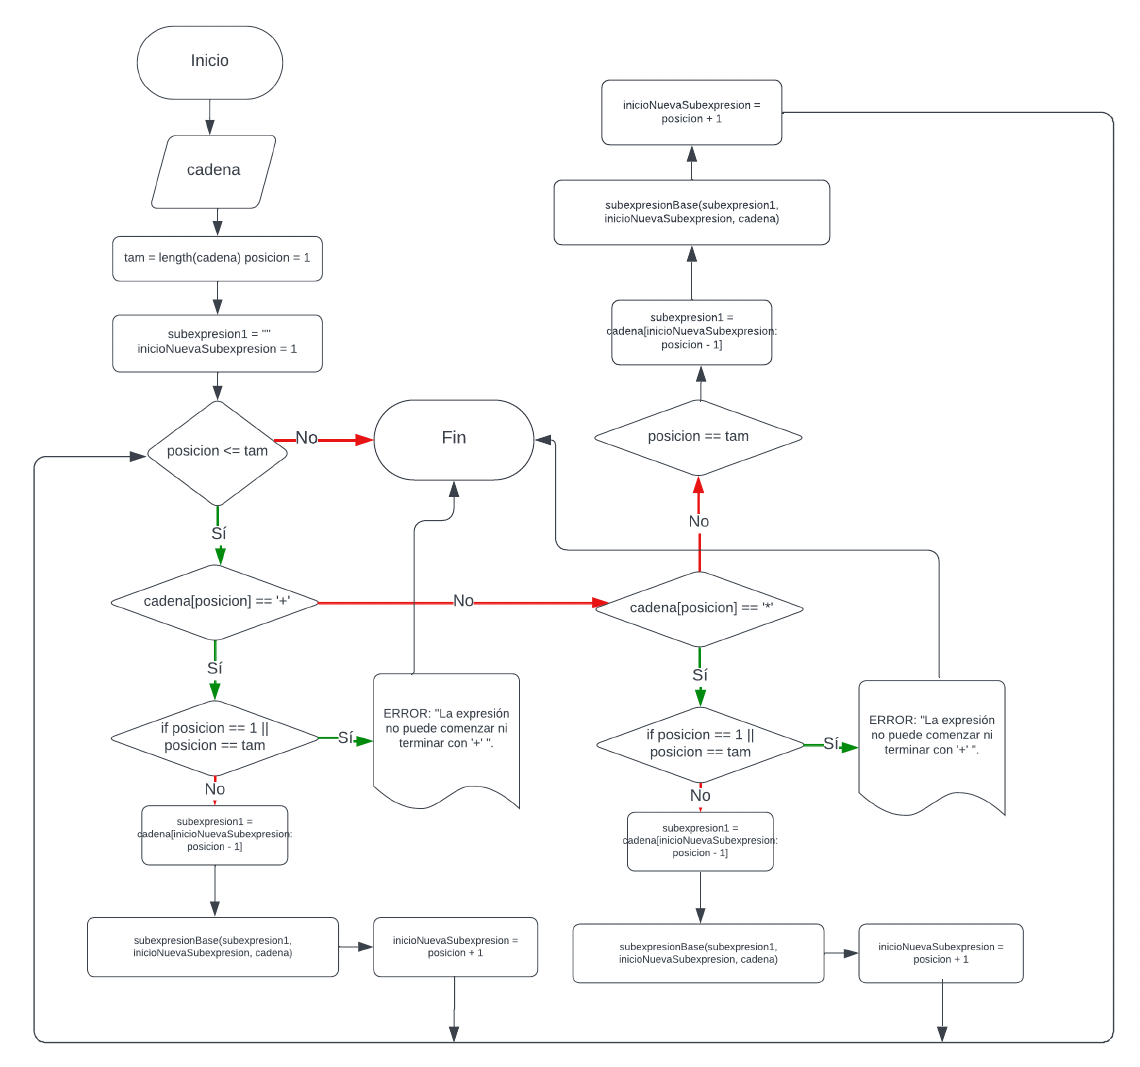
\includegraphics[width=1.255\linewidth]{Función subexpresionesNoVacias.png}
	\label{fig:Gráfica 3}
\end{figure}

\pagebreak
\subsection{Función interpreteAritmético()}
\begin{figure}[h] 
	\centering 	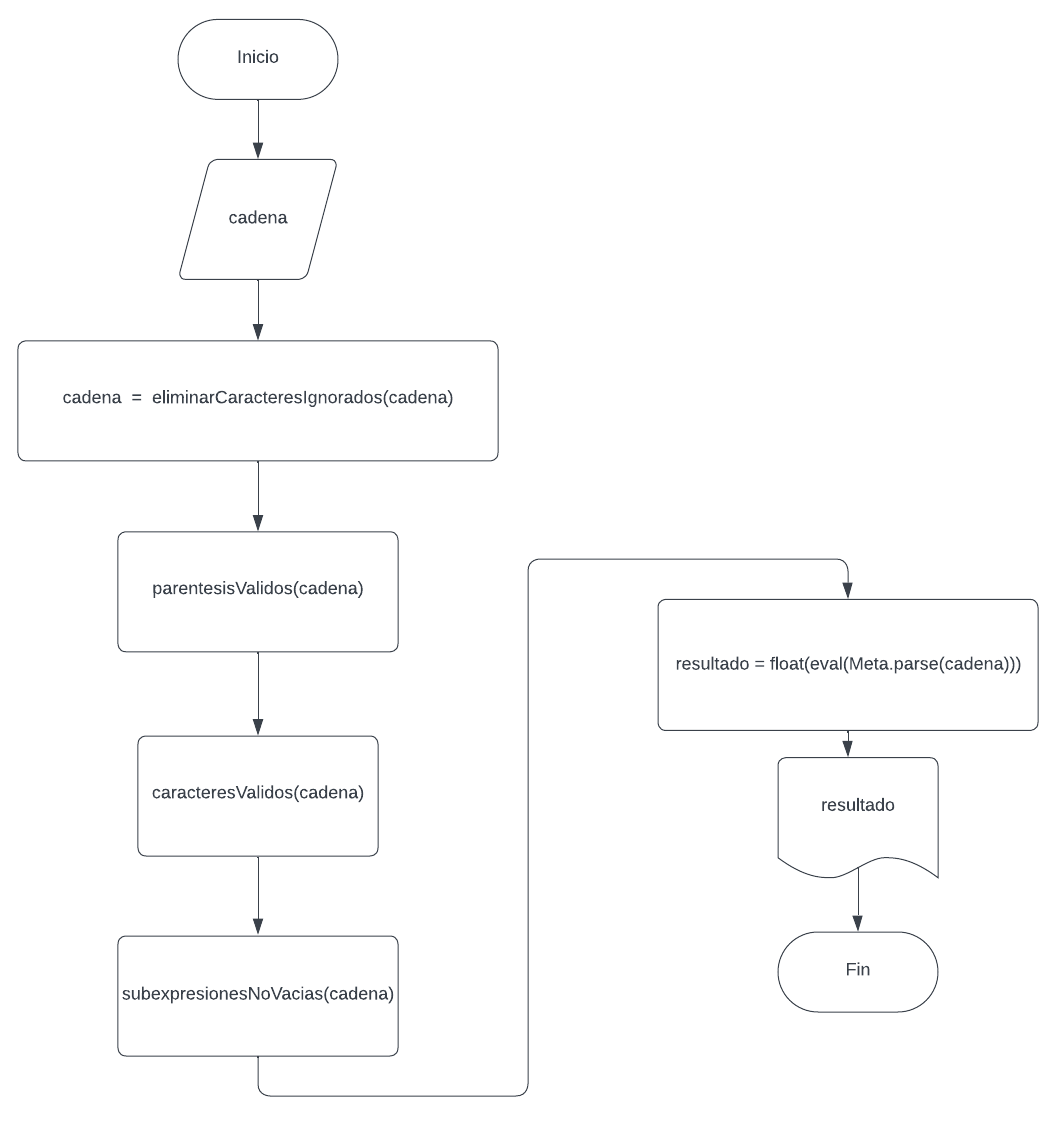
\includegraphics[width=1.1\linewidth]{Función interpreteAritmetico.png}
	\label{fig:Gráfica 3}
\end{figure}

\pagebreak
\subsection{Función entrada()}
\begin{figure}[h] 
	\centering 	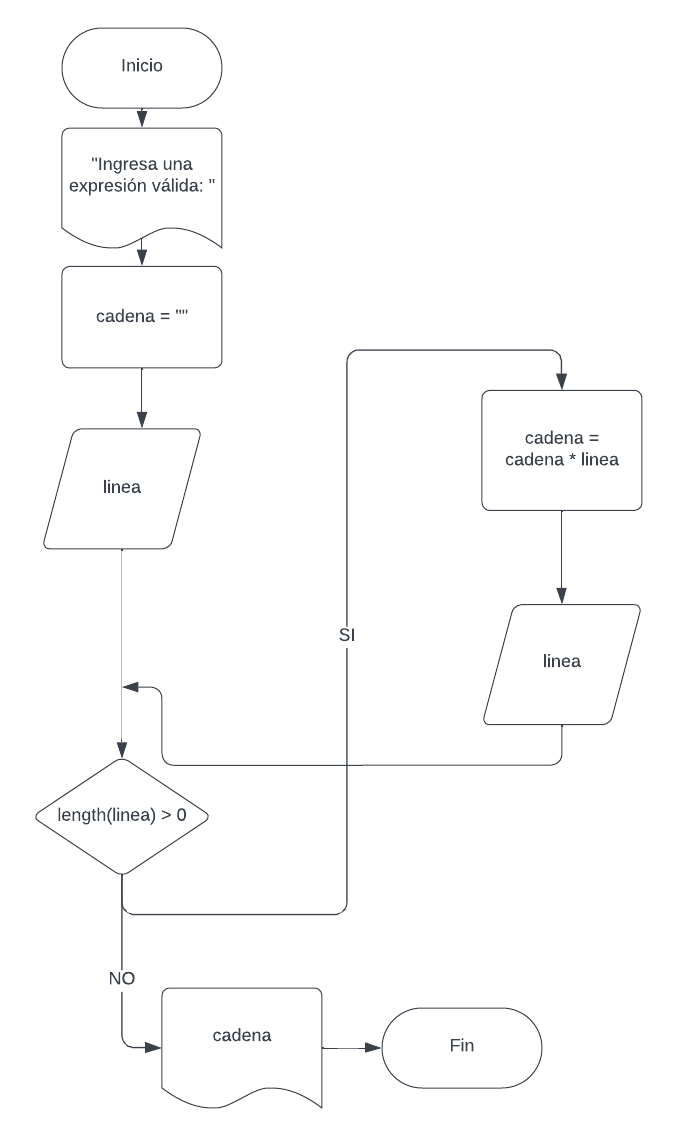
\includegraphics[width=0.7\linewidth]{Función entrada.png}
	\label{fig:Gráfica 3}
\end{figure}


\pagebreak
\section{Instrucciones para utilizar el programa}
\normalsize Para la utilización de nuestro programa se tienen que realizar los siguientes pasos:
\begin{enumerate}
    \item Descargar desde GitHub los archivos en la carpeta de nuestro equipo, dichos archivos van a llevar por nombre:
    \begin{itemize}
        \item interprete\_aritmetico-funciones.jl
        \item interprete\_aritmetico.jl
    \end{itemize}
    \item Una vez descargados, se va a ingresar a julia en alguna aplicación de programación o bien en la máquina virtual.
    \item Tenemos que incluir el archivo interprete\_aritmetico.jl a julia.
    \item Una vez que ya esta incluido automáticamente se va a iniciar el programa, donde se te mencionará qué es y los requisitos que tiene que cumplir la expresión que quieras analizar.
    \item Finalmente, eres libre de usar nuestro intérprete aritmético para sacar el valor de alguna operación con suma o multiplicación .
\end{enumerate}
\large \textbf{CONSIDERACIONES IMPORTANTES:}
\normalsize
\begin{itemize}
    \item Se debe llamar la función en cada ocasión que se quiera usar.
    \item Para mandar a analizar la operación deseada se debe dar doble click, de lo contrario se considera que el usuario quiere ingresar otra línea.
    \item En caso de haber error se va a marcar entre "$<$" y "$>$".
    \item Si el resultado es entero, lo devuelve con terminación .0.
\end{itemize}

\end{document}
